\section{Results}
\label{sec:results}

We now provide a comprehensive view of the timescales that drive the interactions between nearest neighbors, as well as an analysis of the relative velocity, $\textbf{w}_p^\text{nst}$, measured in the DNS.

\subsection{The relative velocity}

As it will be useful for scaling purposes we display on \ref{fig:Reall} the ensemble-averaged \textit{Reynolds} numbers for all the DNS presented in this study.
Formally, we define this \textit{Reynolds} number as
\begin{align*}
    Re = \frac{\rho_f U d}{\mu_f} && \text{with} && U = \textbf{u}_p - \textbf{u}_f
\end{align*}
where $\textbf{u}_f$ is the continuous phase velocity, averaged over the volume occupied by this phase and over all simulation time. 
\begin{figure}[h!]
    \centering
    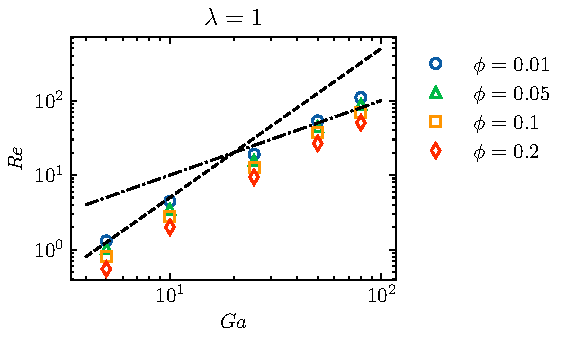
\includegraphics[height = 0.25\textwidth]{image/HOMOGENEOUS_final/CA/Re_l_1.pdf}
    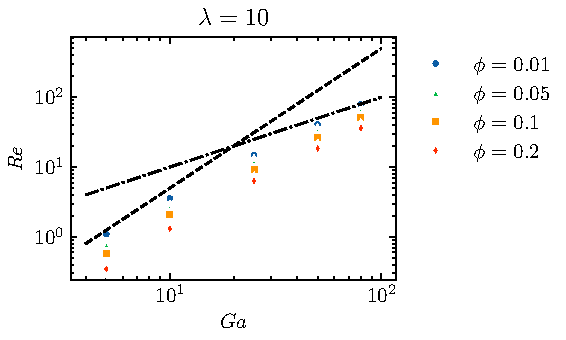
\includegraphics[height = 0.25\textwidth]{image/HOMOGENEOUS_final/CA/Re_l_10.pdf}
    \caption{
        Averaged Reynolds number based on the averaged drift velocity, $Re = \rho_f U d /\mu_f$, with $U = |\textbf{u}_p - \textbf{u}_f|$.
        $\textbf{u}_p$ and $\textbf{u}_f$ are the particle and fluid phase volume and time-averaged velocity.
        (dashed line) $Re \sim Ga^2$ (dot dashed line) $Re \sim Ga$. 
    }
    \label{fig:Reall}
\end{figure}
It is observed that for low $Ga$ the relative velocity scales approximately as $\sim Ga^2$, regardless of the volume fraction $\phi$ and viscosity ratio $\lambda$. 
Note that the \textit{Reynolds} number is globally higher for $\lambda  =1$ and $\lambda = 10$ at $Ga$ and $\phi$ fixed. 
Also, the \textit{Reynolds} number increases with decreasing volume fraction. 
Now that the global absolute kinematics are stated we can analyze pair kinematics. 

% Additionally, let us define the particle phase granular temperature or velocity fluctuation tensor as,
% \begin{equation*}
%     \avg{\delta_i \textbf{u}_i'\textbf{u}_i'}(\textbf{x},t)=
%     \frac{1}{n_p(\textbf{x},t)} 
%     \int \sum_{i}^{N_b}\delta[\textbf{x}-\textbf{x}_i(t,\FF)]  
%     \textbf{u}_i\textbf{u}_i(t,\FF)
%     d\mathscr{P}
%     - n_p \textbf{u}_p \textbf{u}_p,
% \end{equation*}
% The trace of this tensor gives us the granular temperature, namely, 
% \begin{equation*}
%     k_p = \frac{1}{2} \avg{\delta_i\textbf{u}_i'\cdot \textbf{u}_i'}-n_p\textbf{u}_p\cdot \textbf{u}_p
% \end{equation*}
% \begin{figure}[h!]
%     \centering
%     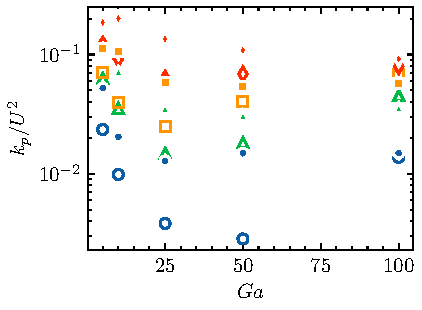
\includegraphics[height = 0.3\textwidth]{image/HOMOGENEOUS_NEW/PA/Talpha.pdf}
%     % 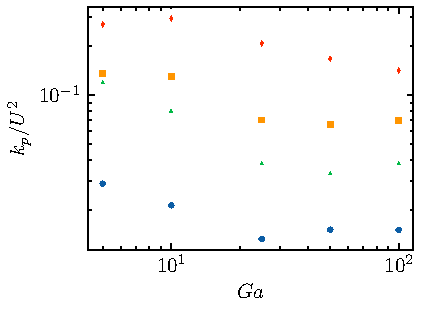
\includegraphics[height = 0.3\textwidth]{image/HOMOGENEOUS_NEW/PA/Talpha_l_10.pdf}
%     \caption{
%         Ensemble averaged granular temperature divided by the mean relative phase velocity,  $k_p = \frac{1}{2}\avg{\delta_i \textbf{u}'_i \textbf{u}_i'}/U^2$ as a function of the Galileo number.  
%         ($\pmb\bigcirc$) $\phi = 0.01$; ($\pmb\triangle$) $ \phi = 0.05$; ($\pmb\square$) $\phi = 0.1$ ($\pmb\lozenge$) $\phi = 0.2$. 
%         The hollow symbols correspond to $\lambda = 1$, the filled symbols to $\lambda = 10$.
%     }
%     \label{fig:Reall}
% \end{figure}
% We display on \ref{fig:Reall} the values of the granular temperature for all our DNS. 
% It is shown that the dimensionless granular temperature increase with $\phi$ at $\lambda$ fixed and is non-monotonic with $Ga$. 
% Additionally, one can note that The value of $k_p/U^2$ globally increase with $\lambda$. 
% The relative velocity and the granular temperature both represent an averaged representation of the particle phase kinematics. 
% The granular temperature measure indirectly the relative motion between particles however it is hard to 

\subsection{Mean age of interaction}

Now, we propose to evaluate the age distribution $P_a$ and to verify the \textit{random destruction assumption} stated in \ref{sec:Theory}. 

In \ref{fig:age_picture} we display the dimensionless age distribution $P_a(a)$, measured in our DNS. 
The age is made dimensionless using the timescale, $U/d_p$ with $d_p = n_p^{-1/3}$.
It is shown in the next few paragraphs that $d_p$ is a representative inter-droplet length scale. 
The theoretical prediction for the age distributions, $P_a(a)$, are obtained by computing the mean \textit{age} $a_p$ from our DNS and using \ref{eq:Pa}. 
The values of $a_p$ are displayed in \ref{fig:tau_p} and will be discussed hereafter. 

It is seen on \ref{fig:age_picture} (right) that the age distributions of the inertial cases are rather well represented by the theoretical age distributions from \ref{eq:Pa}.
Consequently, the \textit{random destruction assumption} holds for the inertial cases. 
Additionally, we see that the distributions spread as the volume fraction decreases.
\begin{figure}[h!]
    \centering
    % 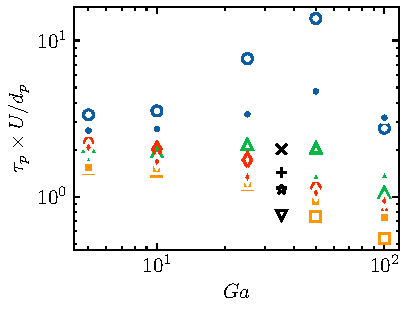
\includegraphics[height = 0.3\textwidth]{image/HOMOGENEOUS_NEW/tau_Ga.pdf}
    % 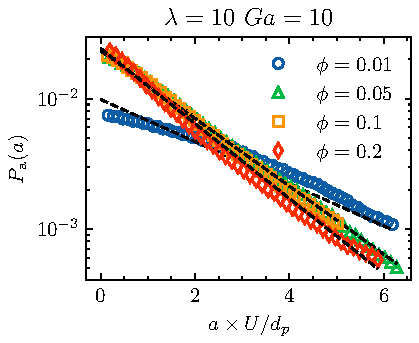
\includegraphics[height = 0.3\textwidth]{image/HOMOGENEOUS_NEW/Dist/Pa_l_10_Ga_10.pdf}
    % 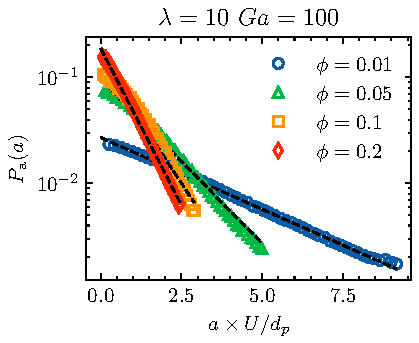
\includegraphics[height = 0.3\textwidth]{image/HOMOGENEOUS_NEW/Dist/Pa_l_10_Ga_100.pdf}
    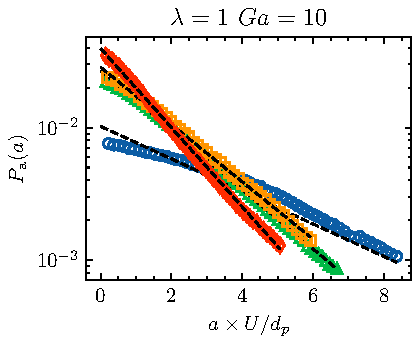
\includegraphics[height = 0.3\textwidth]{image/HOMOGENEOUS_NEW/Dist/Pa_l_1_Ga_10.pdf}
    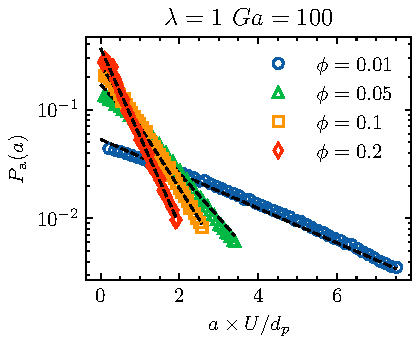
\includegraphics[height = 0.3\textwidth]{image/HOMOGENEOUS_NEW/Dist/Pa_l_1_Ga_100.pdf}
    \caption{
    Age distribution function $P_a(a)$ in terms of the dimensionless age, for $\lambda = 1$.
    (dashed lines) Theoretical age distributions, computed based on the mean age, see \ref{eq:Pa}. 
    The ages are made dimensionless using the relative velocity $U$ and the droplet length scale $d_p = n_p^{-1/3}$.  
    (right) High inertia effects ($Ga = 100$),
    (left) Low inertia effects ($Ga = 10$),
    }
    \label{fig:age_picture}
\end{figure}
In \ref{fig:age_picture} (left)  we provide the age distributions for $Ga = 10$. 
It is seen that the age distribution is well described by \ref{eq:Pa} for $\phi \le 0.05$.
However, for $\phi = 0.01$ we observe that the predicted values of $P_a$ are higher than the DNS results for small ages and smaller for high ages. 
Therefore, at low \textit{Galileo} and low $\phi$ the \textit{random destruction assumption} doesn't seem to remain valid. 
As mentioned earlier the \textit{random destruction assumption} must hold for flows with high droplet velocity fluctuations, since it induces randomness among the droplet interactions \citep{zhang2023evolution} and the interaction history is not important.  
It is clear that for $\phi \to 0$ and $Re \to 0$, the dispersed phase fluctuation also tends to $0$, making this condition harder to meet. 
No differences on $P_a$ are observed when $\lambda = 10 $ therefore we do not display the graphs. 
Anyhow, apart from the dilute and low inertia cases, it is reasonable to say that \ref{eq:Pa} is representative of the age distribution function obtained by DNS.
Consequently, according to \ref{eq:Pa} and \ref{eq:a_p2} the averaged duration of interaction is equivalent to the inverse of the mean destruction rate, that is $\tau_p = a_p$. 

Now let's investigate the value of $a_p$ for all our DNS cases. 
In \ref{fig:tau_p} we display the dimensionless mean age for all our numerical experiments. 
\begin{figure}[h!]
    \centering
    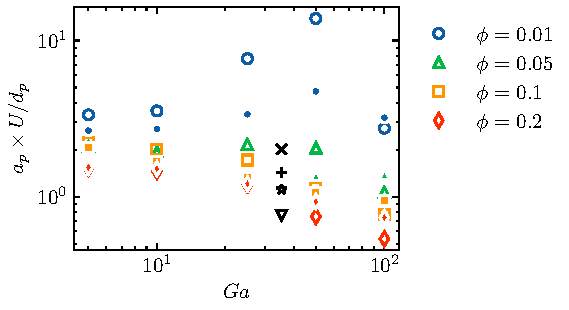
\includegraphics[height = 0.3\textwidth]{image/HOMOGENEOUS_NEW/PA/age.pdf}
    % 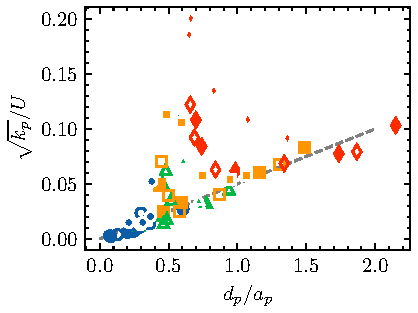
\includegraphics[height = 0.3\textwidth]{image/HOMOGENEOUS_NEW/PA/Corr.pdf}
    % 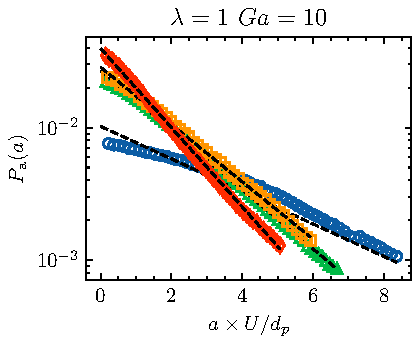
\includegraphics[height = 0.3\textwidth]{image/HOMOGENEOUS_NEW/Dist/Pa_l_1_Ga_10.pdf}
    % 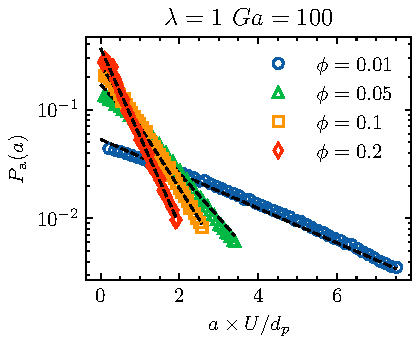
\includegraphics[height = 0.3\textwidth]{image/HOMOGENEOUS_NEW/Dist/Pa_l_1_Ga_100.pdf}
    \caption{
    (left) Mean dimensionless age $\tau_a =  \int_0^\infty aP_a(\textbf{x},t,a)da$ in terms of the \textit{Galileo} number for different volume fraction :   
    ($\pmb\bigcirc$) $\phi = 0.01$; ($\pmb\triangle$) $ \phi = 0.05$; ($\pmb\square$) $\phi = 0.1$ ($\pmb\lozenge$) $\phi = 0.2$.
    The hollow symbols correspond to $\lambda = 1$, the filled symbols to $\lambda = 10$.
    Black symbols represent the DNS results of \citet{zhang2023evolution} for hard sphere suspensions with $\phi = 0.0168,0.0565,0.1341,0.2622$, corresponding to the symbols : $\pmb\times, \pmb +, \pmb\star , \pmb\triangledown$, respectively.
    }
    \label{fig:tau_p}
\end{figure}
Let us first comment on the non-dilute cases $\phi\geq 0.05$. 
It seems that $a_p$ scales well with $U/d_p$ for this range of volume fractions since its values range between $2$ and $0.5$, which is reasonably close to $1$. 
At low volume fraction, it is observed that $a_p$ is constant with $Ga$ until $Ga = 50$ where the mean age starts to decrease. 


At low volume fraction, however, $a_p$ is higher and reaches a peak at $\phi=0.01$, $Ga=50$, $\lambda=1$.
This may be correlated with the values of $A_{xx}$ on \ref{fig:A} which also reach a maximum for these parameters. 
Indeed, since $A_{xx}$ is rather high for these simulations, we know that droplets are, on average, in a side-by-side configuration.
The information that $a_p$ is large too indicated that these sides-by-side configuration seems stable for $\lambda = 1$. 
In opposition to $\lambda = 10$ we observe smaller $a_p$ and also smaller $A_{xx}$ at $\phi = 0.01$ and $Ga = 50$, indicating that, on average, the interactions are not as long, while the microstructure is more isotropic. 

The $\pmb\times$ symbol represents DNS conducted by \citet{zhang2023evolution} on the sedimentation of solid spheres in a liquid. 
The mean age measured in their DNS seems to possess even lower $a_p$ at equivalent $\phi$ and $Ga$. 
This suggests that the duration of interaction of solid particles is shorter than the one of viscous droplets ($\lambda = 10$).
Note that the duration of interaction is even shorter for $\lambda = 1$. 
Pair interaction mechanisms have been investigated by \citet{yin2008lattice} when studying spherical bubbles and solid particle suspensions.
They reach the conclusion that the weaker wake generated by bubbles tends to make them spend more time in close horizontal orientations, in opposition to solid spherical particles. 
Thus, this finding strongly supports the previous observation since the mean age for solid particles is lower than for $\lambda = 1$ indicating that the interactions are less stable for the former. 
In summary, the mean age of interaction seems to be a good way to measure the droplet pairs stability since it provides a way to measure their interaction time. 
This time is shorter for increasing $\phi$, and non-monotonic with $\lambda$ and $Ga$. 
And, in the dilute regime ($\phi = 0.01$) $a_p$ seems to decrease with increasing $\lambda$. 

\subsection{Droplets normal approach velocity}

In the next section we will be interested in the velocity fields $\textbf{w}_p^\text{nst}(\textbf{x},\textbf{r},t,a)$ since it appears in the source term $\textbf{W}(\textbf{x},t)$, which is at the origin of the modifications of the microstructure, see \ref{eq:dt_R}. 
To give a simpler representation of $\textbf{w}_p^\text{nst}(\textbf{x},\textbf{r},t,a)$, we first study the normal approach velocity averaged on all relative positions $\textbf{r}$, that is,  
\begin{equation*}
    w_{pn}^aP_a(\textbf{x},t,a)
    = \frac{1}{n_p(\textbf{x},t)}
    \int_{\mathbb{R}^3}
    \frac{\textbf{r}}{r} \cdot \textbf{w}^\text{nst}_p
    P_\text{nst}(\textbf{x},\textbf{r},t,a) d\textbf{r}.
\end{equation*}
In this way, $w^\text{a}_{pn}(\textbf{x},t,a)$ is the average relative normal approach velocity between the nearest pair of droplets of age $a$. 
The superscript $^a$ indicates that $w_{pn}^a$ is conditioned only on the age $a$. 
It represents the average approach velocity from one droplet to its nearest neighbor, measured from the time when the droplets became nearest neighbors, $a=0$.
A sketch of what we mean by ``normal approach relative velocity'' is given \ref{fig:normal_vel_picture} (right). 
\begin{figure}[h!]
    \centering
    % 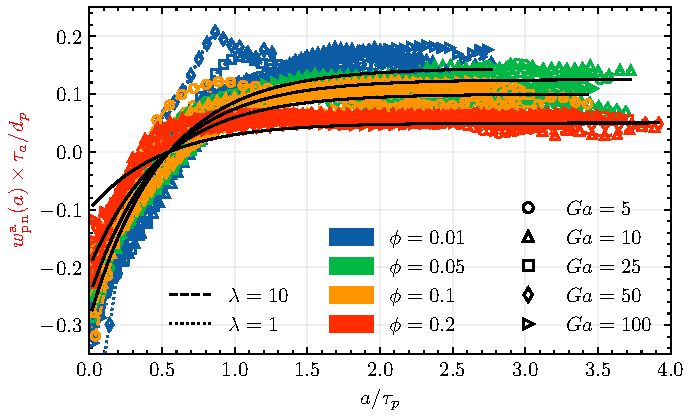
\includegraphics[height = 0.4\textwidth]{image/HOMOGENEOUS_NEW/Age_cond/uR_rel.pdf}
    % \includegraphics[height = 0.3\textwidth]{image/HOMOGENEOUS_NEW/Age_cond/r_l_10_PHI_10.pdf}
    \begin{tikzpicture}[ scale = 0.6]
        \node (img) at (-0.7\textwidth,0){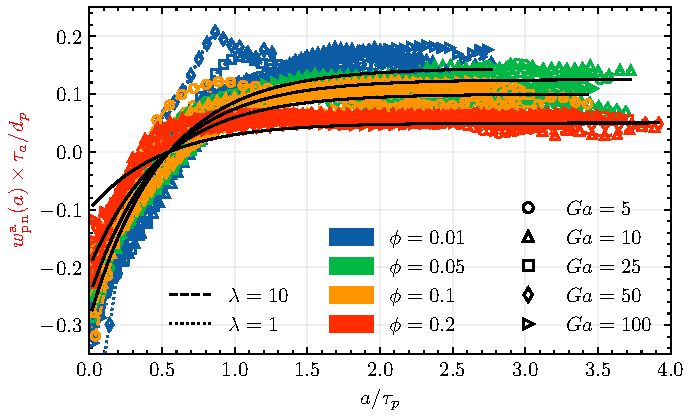
\includegraphics[height = 0.4\textwidth]{image/HOMOGENEOUS_NEW/Age_cond/uR_rel.pdf}};
        \filldraw[ gray!50!white](0,0) circle (0.5);
        \filldraw[ gray!50!white](1,3)circle (0.5);
        % \draw[fill=gray,opacity=0.2](5,-0.2)circle (0.5);
        % \draw[fill=gray,opacity=0.2](-3,2)circle (0.5);
        % \draw[fill=gray,opacity=0.2](-5,0.2)circle (0.5);
        \draw(0,0)node[right]{$\textbf{x}_i$};
        \draw[dashed](0,0)--(1,3)node[right]{$\textbf{x}_j$};
        % \draw[very thick,<-,blue](-1,0)--++(0,1)node[right]{$\bm{b}$};
        \draw[very thick,->](1,3)--++(0.9,-1.8)node[above right]{$\textbf{w}^\text{nst}(a)$};
        \draw[very thick,->,red](1,3)--++(-0.5,-1.5)node[left]{$w_{ij,n}(a)$};
        \draw[dashed](1,3)++(0.9,-1.8) -- (1,3)++(-0.5,-1.5);
        \node (ii) at (1,-1){$\textbf{w}_{ij} = \textbf{u}_j - \textbf{u}_i$};
        \node (ii) at (1,-1.6){$w_{ij,n} = \textbf{w}_{ij}\cdot \textbf{r}/|\textbf{r}|$};
        % \draw[very thick,->](0,0)--++(1,0)node[below right]{$\bm{e_x}$};
        % \draw[very thick,->](0,0)--++(0,1)node[left]{$\bm{e_y}$};
        % \draw(3,1)++(199:1)node[above left]{$\beta$} arc(199:159:1);
        % \draw(0,0)++(0:1)node[above right]{$\theta$} arc(0:20:1);
    \end{tikzpicture} 
    \caption{(left) Relative normal approach velocity between two nearest neighbors, averaged conditionally on the age of interaction.  
    The age $a$, as well as the velocity are made dimensionless  with the mean age $\tau_a$ and the length scale $d_p = n_p^{-1/3}$. 
    % The symbols represent the different \textit{Galileo} numbers, the colors the different 
    % ($\pmb\bigcirc$) $Ga=10$; ($\pmb\triangle$) $ Ga = 25$; ($\pmb\square$) $Ga = 50$ ($\pmb\lozenge$) $Ga =100$.
    % The colors represent the different volume fractions, (blue) $\phi =0.01$, (green) $\phi = 0.05$ (organ) $\phi=0.1$ (red) $\phi = 0.2$. 
    % The white symbols correspond to $\lambda = 1$, and black symbols to $\lambda = 10$. 
    (right)
    Sketch of two nearest neighbors with their position $\textbf{x}_i$ and $\textbf{x}_j$, velocities $\textbf{u}_{i}$ and $\textbf{u}_j$, relative velocity $\textbf{w}_{ij}$ and normal relative velocity $w^{ij,n}$. 
    (black lines) Semi-empirical formulation \eqref{eq:semi-emprical_fits}.
    }
    \label{fig:normal_vel_picture}
\end{figure}
The approach velocity $w_{pn}^a(\textbf{x},t,a)$ for all the DNS carried in this work is displayed \ref{fig:normal_vel_picture} (left). 
The x-axis is made dimensionless with the averaged duration of interaction, $\tau_p$, and the y-axis is scaled with the velocity scale $d_p /\tau_p$. 
At early ages, we observe that $w_{pn}^a<0$.
Then it eventually reaches zero for  $a \approx 0.5\tau_p$.
After this time $w_{pn}^a>0$ and remains constant with respect to $a$. 
Hence, on average, droplets approach each other at early ages ($w_{pn}^a<0$), and then they move apart for $a > \tau_p$ with a constant average velocity.

Two important features are identified from \ref{fig:normal_vel_picture} (left).
First, all curves are roughly similar, even if we can see slight differences in magnitude for the different $\phi$. 
Thus, regardless of the flow parameters, $w_{pn}^a(\textbf{x},t,a)$ scale roughly as $d_p /\tau_p$. 
Second,  $w_{pn}^a(\textbf{x},t,a)$ seems to relax for age, $a > \tau_p$, to reache a constant positive value. 
Consequently, we demonstrated that $\tau_p$ and $d_p$ were the correct time and length scales which govern the inter-droplet scale kinematics, and that $\tau_p$ is also the relaxation time of $w_{pn}^a(\textbf{x},t,a)$. 
In general, we believe that $w_{pn}^a(\textbf{x},t,a)$ may be useful for future studies aiming to construct models based on the relative velocity between droplets \citep{rao2008introduction}. 


We would now like to build a kinetic model for the normal approach velocity of droplets. 
This is of particular interest since closure terms such as collision kernel are directly related to the normal approach velocity between droplets \citep{sundaram1997collision}.
Looking at \ref{fig:normal_vel_picture} we can propose that the normal approach velocity has the form:
\begin{equation}
    w_{pn}^a(\textbf{x},t,a) = \frac{d_p}{\tau_p} \left(
        - C_1 e^{- 2 a/\tau_p }
        + C_2
    \right)
\end{equation}
The theoretical observations made in \ref{sec:Theory} suggest that in a statistically steady-state regime, the normal approach velocity must respect the condition :
\begin{equation}
\int_\mathbb{R} w_{pn}^aP_a(\textbf{x},t,a) da = 0 
\end{equation}
which means that both constants must respect $C_2 = C_1 /3$. 
% Let consider that the maximum value of $w_{pn}^a$ is reached for the lowest volume fraction $\phi = 0.01$ at $a \to \infty$ (see \ref{fig:normal_vel_picture}).     
% Besides approaching the packing volume fraction limit $\phi_\text{max}$ the relative velocity must approach zero. 
Additionally, suppose that $w_{pn}^a(\textbf{x},t,a\to\infty,\phi)$ varies linearly with $\phi$ from $w_{pn}^a(\textbf{x},t,a\to\infty,\phi = 0.01) \approx 0.15$ to $w_{pn}^a(\textbf{x},t,a\to\infty,\phi = 0.2) \approx 0.05$. 
This leads us to $C_2 \approx -1/2 (\phi - 0.01) + 0.01$. 
Note that the dependency of $w_{pn}$ on $Ga$ and $\lambda$ is implicitly included in the mean age.
Making use of all these remarks a consistent model for the relative normal approach velocity is, 
\begin{equation}
    w_{pn}^a(\textbf{x},t,a) = \frac{d_p}{\tau_p} 
    \left(
        0.15
        -\frac{\phi}{2}
    \right)\left(
        1 - 3e^{-2a/\tau_p}
    \right).
   \label{eq:semi-emprical_fits}
\end{equation}
On \ref{fig:normal_vel_picture}, we can observe that the black lines, representing \ref{eq:semi-emprical_fits} for various values of $\phi$, describe relatively well the mean normal approach velocity measured in the DNS. 
Thus, we obtained a reasonable model for $w_{pn}$ in terms of the volume fraction and the mean age of interaction $\tau_p$.
The remaining thing to do would be to create a closed model for $\tau_p$ in terms of $Ga$, $\phi$ and $\lambda$. 
